\documentclass[10pt]{article}
\usepackage{tikz}
\usetikzlibrary{shapes.misc}
\usepackage[margin=0cm]{geometry}
\pagestyle{empty}
\tikzstyle{every node}=[cross out, draw, red]

\begin{document}

\vspace*{\fill}
\begin{center}
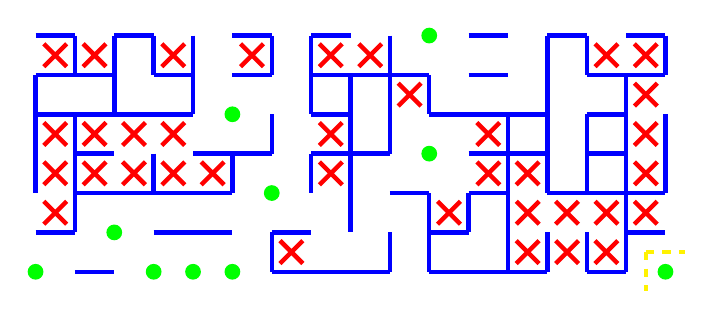
\begin{tikzpicture}[x=0.5cm, y=-0.5cm, ultra thick, blue]
% Walls
    \draw (0,0) -- (1,0);
    \draw (2,0) -- (3,0);
    \draw (5,0) -- (6,0);
    \draw (7,0) -- (8,0);
    \draw (11,0) -- (12,0);
    \draw (13,0) -- (14,0);
    \draw (15,0) -- (16,0);
    \draw (0,1) -- (2,1);
    \draw (3,1) -- (4,1);
    \draw (5,1) -- (6,1);
    \draw (7,1) -- (10,1);
    \draw (11,1) -- (12,1);
    \draw (14,1) -- (16,1);
    \draw (0,2) -- (4,2);
    \draw (7,2) -- (8,2);
    \draw (10,2) -- (13,2);
    \draw (14,2) -- (15,2);
    \draw (1,3) -- (2,3);
    \draw (4,3) -- (6,3);
    \draw (7,3) -- (9,3);
    \draw (11,3) -- (13,3);
    \draw (14,3) -- (15,3);
    \draw (1,4) -- (5,4);
    \draw (9,4) -- (10,4);
    \draw (11,4) -- (12,4);
    \draw (13,4) -- (16,4);
    \draw (0,5) -- (1,5);
    \draw (3,5) -- (5,5);
    \draw (6,5) -- (7,5);
    \draw (10,5) -- (11,5);
    \draw (15,5) -- (16,5);
    \draw (1,6) -- (2,6);
    \draw (6,6) -- (9,6);
    \draw (10,6) -- (13,6);
    \draw (14,6) -- (15,6);
    \draw (0,1) -- (0,4);
    \draw (1,0) -- (1,1);
    \draw (1,2) -- (1,5);
    \draw (2,0) -- (2,2);
    \draw (3,0) -- (3,1);
    \draw (3,3) -- (3,4);
    \draw (4,0) -- (4,2);
    \draw (5,3) -- (5,4);
    \draw (6,0) -- (6,1);
    \draw (6,2) -- (6,3);
    \draw (6,5) -- (6,6);
    \draw (7,0) -- (7,2);
    \draw (7,3) -- (7,4);
    \draw (8,1) -- (8,5);
    \draw (9,0) -- (9,3);
    \draw (9,5) -- (9,6);
    \draw (10,1) -- (10,2);
    \draw (10,4) -- (10,6);
    \draw (11,4) -- (11,5);
    \draw (12,2) -- (12,6);
    \draw (13,0) -- (13,4);
    \draw (13,5) -- (13,6);
    \draw (14,0) -- (14,1);
    \draw (14,2) -- (14,4);
    \draw (14,5) -- (14,6);
    \draw (15,1) -- (15,6);
    \draw (16,0) -- (16,1);
    \draw (16,2) -- (16,4);
% Pillars
    \fill[green] (10,0) circle(0.2);
    \fill[green] (5,2) circle(0.2);
    \fill[green] (10,3) circle(0.2);
    \fill[green] (6,4) circle(0.2);
    \fill[green] (2,5) circle(0.2);
    \fill[green] (0,6) circle(0.2);
    \fill[green] (3,6) circle(0.2);
    \fill[green] (4,6) circle(0.2);
    \fill[green] (5,6) circle(0.2);
    \fill[green] (16,6) circle(0.2);
% Inner points in accessible cul-de-sacs
    \node at (0.5,0.5) {};
    \node at (1.5,0.5) {};
    \node at (3.5,0.5) {};
    \node at (5.5,0.5) {};
    \node at (7.5,0.5) {};
    \node at (8.5,0.5) {};
    \node at (14.5,0.5) {};
    \node at (15.5,0.5) {};
    \node at (9.5,1.5) {};
    \node at (15.5,1.5) {};
    \node at (0.5,2.5) {};
    \node at (1.5,2.5) {};
    \node at (2.5,2.5) {};
    \node at (3.5,2.5) {};
    \node at (7.5,2.5) {};
    \node at (11.5,2.5) {};
    \node at (15.5,2.5) {};
    \node at (0.5,3.5) {};
    \node at (1.5,3.5) {};
    \node at (2.5,3.5) {};
    \node at (3.5,3.5) {};
    \node at (4.5,3.5) {};
    \node at (7.5,3.5) {};
    \node at (11.5,3.5) {};
    \node at (12.5,3.5) {};
    \node at (15.5,3.5) {};
    \node at (0.5,4.5) {};
    \node at (10.5,4.5) {};
    \node at (12.5,4.5) {};
    \node at (13.5,4.5) {};
    \node at (14.5,4.5) {};
    \node at (15.5,4.5) {};
    \node at (6.5,5.5) {};
    \node at (12.5,5.5) {};
    \node at (13.5,5.5) {};
    \node at (14.5,5.5) {};
% Entry-exit paths without intersections
    \draw[dashed, yellow] (15.5,5.5) -- (16.5,5.5);
    \draw[dashed, yellow] (15.5,5.5) -- (15.5,6.5);
\end{tikzpicture}
\end{center}
\vspace*{\fill}

\end{document}
